\documentclass[pdftex,a4paper,12pt]{report}
\newtheorem{theorem}{Theorem}[section]
\newtheorem{lemma}[theorem]{Lemma}
\newtheorem{proposition}[theorem]{Proposition}
\newtheorem{corollary}[theorem]{Corollary}

\newenvironment{proof}[1][Proof]{\begin{trivlist}
\item[\hskip \labelsep {\bfseries #1}]}{\end{trivlist}}
\newenvironment{definition}[1][Definition]{\begin{trivlist}
\item[\hskip \labelsep {\bfseries #1}]}{\end{trivlist}}
\newenvironment{example}[1][Example]{\begin{trivlist}
\item[\hskip \labelsep {\bfseries #1}]}{\end{trivlist}}
\newenvironment{remark}[1][Remark]{\begin{trivlist}
\item[\hskip \labelsep {\bfseries #1}]}{\end{trivlist}}

\newcommand{\qed}{\nobreak \ifvmode \relax \else
      \ifdim\lastskip<1.5em \hskip-\lastskip
      \hskip1.5em plus0em minus0.5em \fi \nobreak
      \vrule height0.75em width0.5em depth0.25em\fi}
\def\therefore{
\leavevmode
\lower0.1ex\hbox{$\bullet$}
\kern-0.2em\raise0.7ex\hbox{$\bullet$}
\kern-0.2em\lower0.2ex\hbox{$\bullet$}
\thinspace}
\usepackage{amsmath}
\usepackage{multicol}
\usepackage{hyperref}
\usepackage{color}
\usepackage{fullpage}
\usepackage{graphicx}
\newcommand{\abs}[1] {$\mid #1 \mid$}
\renewcommand{\thesection}{\arabic{section}}

\hypersetup{
  colorlinks,
  citecolor=blue,
  linkcolor=blue,
  urlcolor=blue
}
\begin{document}
\begin{titlepage}
\begin{center}

\textsc{\LARGE IIT Kanpur}\\[1.5cm]

\textsc{\Large CS345A - AlgorithmsII}\\[0.5cm]

% Title
{ \huge \bfseries Assignment 5 \\[0.4cm] }


\begin{minipage}{0.4\textwidth}
\begin{flushleft} \large
Anjani Kumar\\
11101
\end{flushleft}
\end{minipage}
\begin{minipage}{0.4\textwidth}
\begin{flushright} \large
Sumedh Masulkar\\
11736
\end{flushright}
\end{minipage}

\vfill

% Bottom of the page
{\large March 25, 2014}

\end{center}
\end{titlepage}

\tableofcontents
\newpage

\section{An Atmospheric Science Experiment : Part-1}

\subsection{Instance of max-flow problem corresponding to instance of the given problem}

\begin{figure}[ht!]
\centering
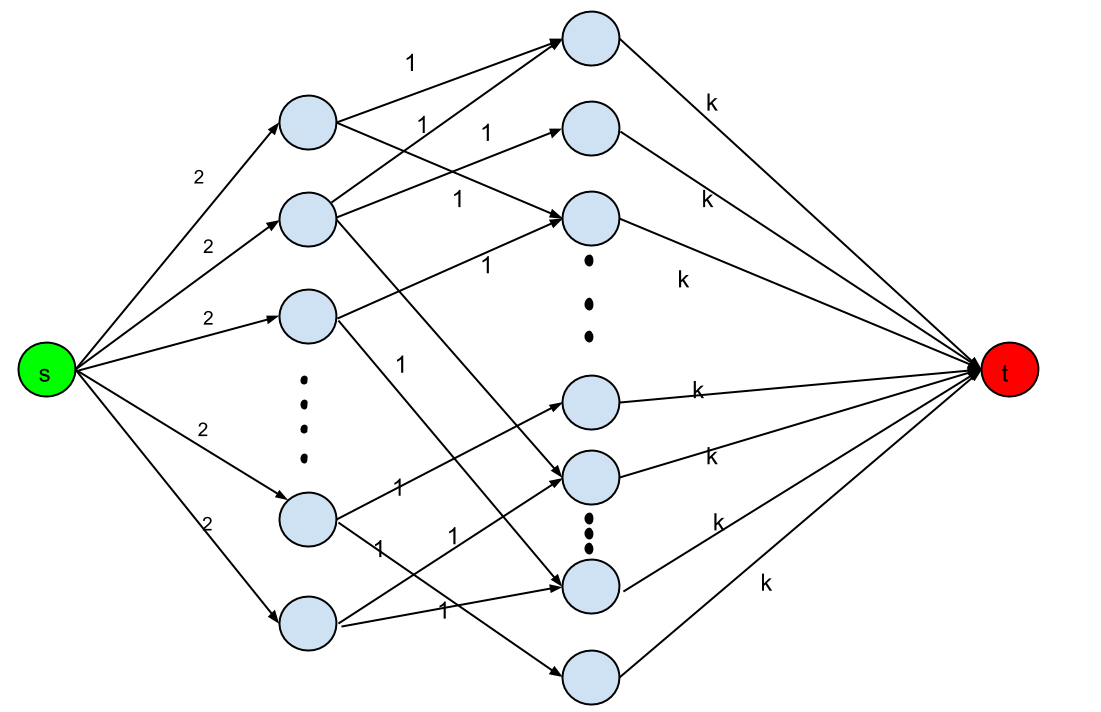
\includegraphics[width=150mm]{fig1.png}
\caption{Figure for part-1}
\label{fig:fig1}
\end{figure}

A directed graph $G$ $=$ ($V,\ E$), where $V$ is the set of vertices, and $E$ is the set of edges of the graph.

\begin{itemize}
 \item \underline{\textbf{$V$}}: The set of vertices of the graph contains,
     \begin{itemize}
     \item A source $s$.
     \item m vertices corresponding to m balloons.
     \item n vertices corresponding to n atmospheric conditions.
     \item A sink $t$.
     \end{itemize}
 \item \underline{\textbf{$E$}}: The edges in the graph are,
     \begin{itemize}
     \item ($s$, $i$), $\forall$ $i$ $\in$ m vertices(corresponding to balloons), $s$ is the source,\\and capacity($s$, $i$) $=$ 2.
     \item ($i$, $j$), $\forall$ $i$ $\in$ m vertices(corresponding to balloons) to $j$, $\forall$ $j$ $\in$ $S_i$. Here edge capacity for all ($i$, $j$) $=$ 1.
     \item ($j$, $t$), $\forall$ $j$ $\in$ n vertices(corresponding to conditions), $t$ is the sink,\\and capacity($j$, $t$) $=$ $k$.
     \end{itemize}
\end{itemize}

\subsection{Theorem}

There is a way to measure each condition by $k$ different balloons, while each balloon only measures at most two conditions \textbf{iff} the value of maximum flow from $s$ to $t$ is $nk$.

\subsection{Proof}

\begin{itemize}
\item \textbf{\underline{Proof for ($=>$)}}: If there is a way to measure each condition by $k$ different balloons, while each balloon measures at most two conditions, for given $n$ conditions, the sets $S_i$ for each of the m balloons and $k$, then the value of maximum flow from $s$ to $t$ in $G$ must be $nk$.
\paragraph{Proof:} \makebox[2pt]{}\\\\
Let $A$ be the set of m vertices corresponding to the balloons and $B$ be the set of n vertices corresponding to the conditions.\\
Thus, $\mid A \mid$ $=$ m, and $\mid B \mid$ $=$ n.\\\\
Let $S$ be a way to measure each condition by $k$ different balloons while each balloon measures at most two conditions. Let $S_j$ be the set of $k$ balloons measuring condition $j$ $\in$ $B$.
\paragraph{Construction of corresponding max-flow:} 
    \begin{itemize}
    \item For each ($j$, $t$), where $j\ \in\ B$, assign flow from $j$ to $t$ to $k$.
    \item For each ($i$, $j$), where $j\ \in\ B$, and $i\ \in\ S_j$, assign flow from $i$ to $j$ to 1.
    \item For each ($s$, $i$), where $i\ \in\ A$, assign flow from $s$ to $i$ to $\sum _j flow(i,\ j)$ where $j\ \in\ B$.
    \end{itemize}

\paragraph{Validity of constraints}:
\begin{itemize}
\item \textbf{\underline{Capacity constraints:}}
    \begin{itemize}
    \item For each ($s$, $i$), where $i\ \in\ A$, $flow$($s$, $i$) $=$ $\sum _j flow(i,\ j)$ $\leq$ 2 $=$ $capacity$($s$, $i$).
    \item For each ($i$, $j$), if balloon $i$ measures condition $j$, then $flow$($s$, $i$) $=$ 1, otherwise 0. Thus, $flow$($s$, $i$) $\leq$ $capacity$($i$, $j$).
    \item For each ($j$, $t$), $flow$($j$, $t$) $=$ $k$ $=$ $capacity$($j$, $t$).
    \item Thus, all capacity constraints are satisfied.
    \end{itemize}
\item \textbf{\underline{Conservation constraints:}}
    \begin{itemize}
    \item The only intermediate vertices are $A \cup B$.
    \item For each vertex $i$ in $A$, $f_{in}(i)$ $=$ $f_{out}(i)$ $=$ $\sum _j flow(i,\ j)$ where $j\ \in\ B$.
    \item For each vertex $j$ in $B$, $f_{in}(j)$ $=$ $k$, since $k$ balloons measure condition $j$. Also, $f_{out}(j)$ $=$ $k$.
    \item Thus, $f_{in}(j)$ - $f_{out}(j)$ $=$ 0 $\forall$ $u\ \in\ V-$\{$s,\ t$\}.
    \end{itemize}
\end{itemize}

We know that value of max flow in $G$ $\leq$ $nk$, since $\mid B \mid$ $=$ n, and $f_{out}(j)$ for each $j\ \in\ B$ $=$ k.\\\\
Also, as per flows constructed above, value of flow $=$ $nk$(Thus, it is the max-flow possible).

\item \textbf{\underline{Proof for ($<=$)}}: If the value of maximum flow from $s$ to $t$ in $G$ is $nk$, then there exists a way to measure each condition according to given constraints.
\paragraph{Proof:}
\begin{itemize}
\item For each ($s$, $i$), where $i\ \in\ A$, capacity is 2, hence balloon $i$ can measure at most 2 conditions.
\item For each ($i$, $j$), where $i\ \in\ A$, and $j\ \in\ B$, capacity is 1, thus ensuring a balloon doesn't measure same condition twice. Since, flow is $nk$, there will be $k$ $i$ with flow 1 on a given $j$.
\item For each ($j$, $t$), where $j\ \in\ B$, capacity is $k$, hence ensuring one condition is measured by at most $k$ balloons.
\item Thus, we can see this is a solution of the problem satisfying all constraints.
\end{itemize}
\end{itemize}

\section{An Atmospheric Science Experiment : Part-2}

\subsection{Instance of max-flow problem corresponding to instance of the given problem}

\begin{figure}[ht!]
\centering
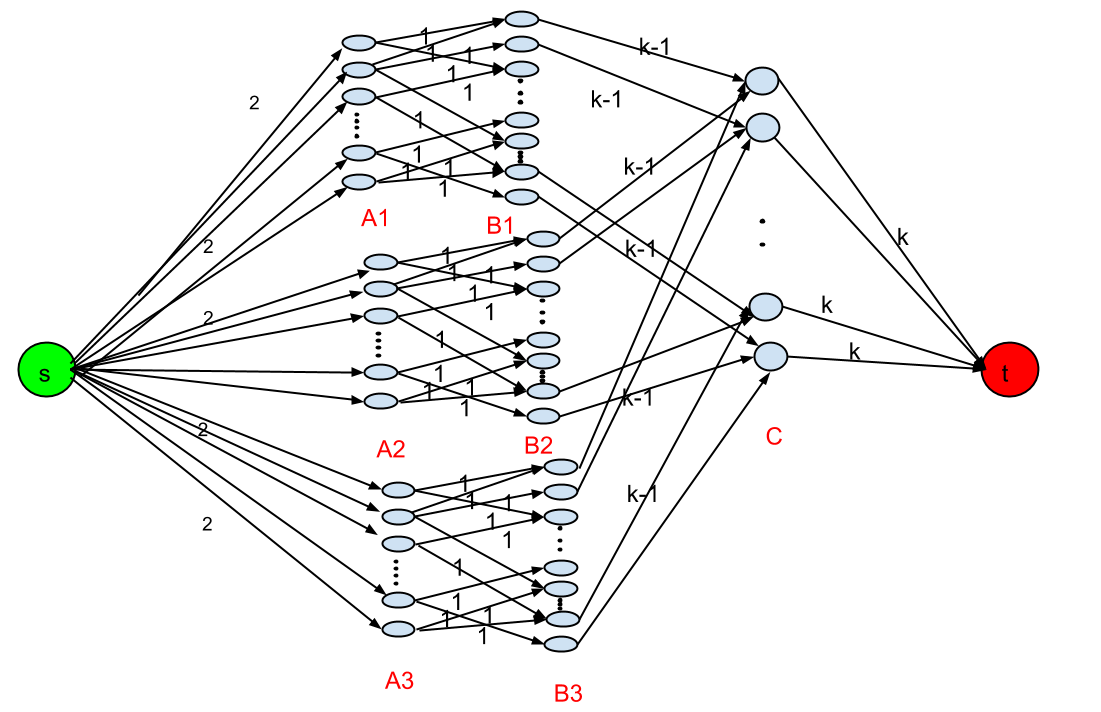
\includegraphics[width=150mm]{fig2.png}
\caption{Figure for part-2}
\label{fig:fig2}
\end{figure}

A directed graph $G$ $=$ ($V,\ E$), where $V$ is the set of vertices, and $E$ is the set of edges of the graph.

\begin{itemize}
 \item \underline{\textbf{$V$}}: The set of vertices of the graph contains,
     \begin{itemize}
     \item A source $s$.
     \item 3 set of vertices, $A1,\ A2,\ A3$ corresponding to balloons from three contractors such that $\mid A1 \mid\ +\ \mid A2 \mid\ +\ \mid A3 \mid$ $=\ m$.
     \item 3 set of n vertices, $B1,\ B2,\ B3$ corresponding to conditions for different contractors.
     \item $n$ vertices corresponding to each condition(set $C$).
     \item A sink $t$.
     \end{itemize}
 \item \underline{\textbf{$E$}}: The edges in the graph are,
     \begin{itemize}
     \item ($s$, $i$), $\forall$ $i$ $\in$ $A1,\ A2,\ A3$(corresponding to balloons), $s$ is the source,\\and capacity($s$, $i$) $=$ 2.
     \item ($i$, $j$), $\forall$ $i$ $\in$ $A1$ to $j$ $\in$ $B1$, $\forall$ $i$ $\in$ $A2$ to $j$ $\in$ $B2$, $\forall$ $i$ $\in$ $A3$ to $j$ $\in$ $B3$. Here all edges have capacity 1.
     \item ($j$, $l$), $i^{th}$ vertex of each $B_x$(x$=$1,2,3) maps to $i^{th}$ vertex of $C$, with capacity of each edge $k\ -\ 1$.
     \item ($l$, $t$), $\forall$ $l$ $\in$ $C$, $t$ is the sink, and capacity($l$, $t$) $=$ $k$.
     \end{itemize}
\end{itemize}

\subsection{Theorem}

There is a way to measure each condition by $k$ different balloons, while each balloon only measures at most two conditions and no condition exists such that all k measurements come from balloons produced by a single contractor \textbf{iff} the value of maximum flow from $s$ to $t$ is $nk$.

\subsection{Proof}

\begin{itemize}
\item \textbf{\underline{Proof for ($=>$)}}: If there is a way to measure each condition by $k$ different balloons, while each balloon measures at most two conditions and no condition exists such that all k measurements come from balloons produced by a single contractor, for given $n$ conditions, the sets $S_i$ for each of the m balloons and $k$, then the value of maximum flow from $s$ to $t$ in $G$ must be $nk$.
\paragraph{Proof:} \makebox[2pt]{}\\\\
Let $S$ be a way to measure each condition by $k$ different balloons while each balloon measures at most two conditions and no condition exists such that all k measurements come from balloons produced by a single contractor. Let $S_l$ be the set of $k$ balloons measuring condition $l$ $\in$ $C$.
\paragraph{Construction of corresponding max-flow:} 
    \begin{itemize}
    \item For each ($l$, $t$), where $l\ \in\ C$, assign flow from $l$ to $t$ to $k$.
    \item For each ($i$, $j$), where $j\ \in\ B_x$, where ($1 \leq x \leq 3$), and $i\ \in\ S_l$, assign flow from $i$ to $j$ to 1. To the remaining $i$ $\in$ $B1 \cup B2 \cup B3$, assign flow from $i$ as 0.
    \item For each ($s$, $i$), where $i\ \in\ A_x$, assign flow from $s$ to $i$ to $\sum _j flow(i,\ j)$ where $j\ \in\ B_x$ and $1 \leq x \leq 3$.
    \item For each ($j$, $l$), where $j\ \in\ B_x$ and $1 \leq x \leq 3$ and $l\ \in\ C$, assign flow from $j$ to $l$ to $\sum _j flow(i,\ j)$ where $i\ \in\ A_x$.
    \end{itemize}

\paragraph{Validity of constraints}:
\begin{itemize}
\item \textbf{\underline{Capacity constraints:}}
    \begin{itemize}
    \item For each ($s$, $i$), where $i\ \in\ A$, $flow$($s$, $i$) $=$ $\sum _j flow(i,\ j)$ $\leq$ 2 $=$ $capacity$($s$, $i$).
    \item For each ($i$, $j$), if balloon $i$ measures condition $j$, then $flow$($s$, $i$) $=$ 1, otherwise 0. Thus, $flow$($s$, $i$) $\leq$ $capacity$($i$, $j$).
    \item For each ($j$, $l$), where $l$ $\in$ $C$, flow $\leq$ k$-$1 = capacity of the edge.
    \item For each ($l$, $t$), $flow$($l$, $t$) $=$ $k$ $=$ $capacity$($l$, $t$).
    \item Thus, all capacity constraints are satisfied.
    \end{itemize}
\item \textbf{\underline{Conservation constraints:}}
    \begin{itemize}
    \item The only intermediate vertices are $A_x \cup B_x \cup C$ and $1 \leq x \leq 3$.
    \item For each vertex $i$ in $A_x$, $f_{in}(i)$ $=$ $f_{out}(i)$ $=$ $\sum _j flow(i,\ j)$ where $j\ \in\ B_x$.
    \item For each vertex $j$ in $B_x$, $f_{in}(j)$ $=$ $\sum _j flow(i,\ j)$ where $i$ in $A_x$.
    \item For each $l$ $\in$ $C$, $f_{out}(l)\ =\ k$, and $f_{out}(l)\ =\ =\ sum _j flow(i,\ j)\ k$, since $S$ is a solution.
    \item Thus, $f_{in}(j)$ - $f_{out}(j)$ $=$ 0 $\forall$ $u\ \in\ V-$\{$s,\ t$\}.
    \end{itemize}
\end{itemize}

We know that value of max flow in $G$ $\leq$ $nk$, since $\mid C \mid$ $=$ n, and $f_{out}(l)$ for each $l\ \in\ C$ $=$ k.\\\\
Also, as per flows constructed above, value of flow $=$ $nk$(Thus, it is the max-flow possible).

\item \textbf{\underline{Proof for ($<=$)}}: If the value of maximum flow from $s$ to $t$ in $G$ is $nk$, then there exists a way to measure each condition according to given constraints.
\paragraph{Proof:}
\begin{itemize}
\item For each ($s$, $i$), where $i\ \in\ A_x$, capacity is 2, hence balloon $i$ can measure at most 2 conditions.
\item For each ($i$, $j$), where $i\ \in\ A_x$, and $j\ \in\ B_x$, capacity is 1, thus ensuring a balloon doesn't measure same condition twice.
\item For each ($j$, $l$), capacity of the edge is $k-1$, ensuring all $k$ balloons are not from the same contractor.
\item For each ($l$, $t$), where $l\ \in\ C$, capacity is $k$, hence ensuring one condition is measured by at most $k$ balloons.
\item Thus, we can see this is a solution of the problem satisfying all constraints.
\end{itemize}
\end{itemize}
\newpage

\section{Job Scheduling using Max-Flow}
\subsection{Problem}
Each job j has an arrival time $a_j$ when it is first available
for processing, a length $l_j$ which indicates how much processing time it needs and a deadline $d_j$ by which it must be finished. ($0 \leq j \leq d_j\ -\ a_j$ .) Each job can be run on any of the
processors, but only on one at a time; it can also be preempted and resumed from where it left off (possibly after a delay).
Moreover, the collection of processors is not entirely static either: you have an overall pool of k possible
processors; but for each processor $i$ there is an interval of time [$t_i, t'_i$] during which it is available; it is unavailable at all other times.
Given all this data about job requirement and processor availability, we have to decide whether the jobs can all be completed or not. 
\subsection{An Instance of the Max-Flow problem:}
\begin{center}
\begin{figure}[ht!]
\centering
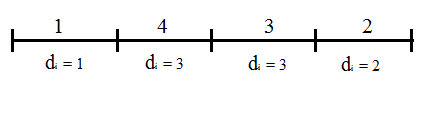
\includegraphics{fig3.jpg}
\caption{A graph representing the Max-Flow diagram of the instance.}
\label{fig:2.1}
\end{figure}
\end{center}
\textbf{Salient features of the graph:}
\begin{itemize}
\item $l_i$ is the length of the $i^{th}$ job.
\item $i_j$ is the length of the $j^{th}$ interval.
\item $n_j$ is the number of processors active during the $j^{th}$ interval.
\end{itemize}
\begin{center}
\begin{figure}[ht!]
\centering
\includegraphics{fig4.jpg}
\caption{Distribution of Intervals:An Interval timeline}
\label{fig:2.2}
\end{figure}
\end{center}
\textbf{Salient Points for creating intervals}
\begin{itemize}
\item Plot the times $a_j,d_j$ $\forall$ job $j$ and $t_i,t'_i$ $\forall$ processor $i$ on a horizontal axis.
\end{itemize}
\textbf{Validity of the interval set}\\
The proposed interval distribution is valid because a job can be preempted only in the following 3 cases:
\begin{itemize}
\item A new job is to be processed.
\item Deadline of the on-going job has been reached.
\item The current job has been completed.
\item A processor has completed its tenure or a new one enters for scheduling.
\end{itemize}
Since the distribution is done keeping the above cases in mind, the proposed distribution scheme is valid.\\
\textbf{Construction of the Network Flow graph:}\\
\begin{itemize}
\item insert a start point $s$, all the $n$ jobs, all the intervals $i$ and an end point $t$.
\item Create an edge from $s$ to job $j_i$ with capacity $l_i\ \forall$ jobs in the job set.
\item Create an edge from each job $j$ in the job set to each interval set node $i$ whose interval lies within $a_j$ and $d_j$; with the capacities being the length($i_i$) of the intervals. 
\item Create an edge from interval set node $i$ to end point $f\ \forall$ intervals; with capacity of edge being $i_i*n_i$. where $i_i\ =$ length of interval $i$ and $n_i\ =$ number of processor active during the $i^{th}$ interval.
\end{itemize}

        
\subsection{Theorem}
\begin{center}
All the jobs can be scheduled before their deadline, \textbf{if and only if} $\exists$ a \textbf{maximum flow} from $s$ to $t$ of value $\sum_{i=1}^{n}\ l_i$ where $n\ =$ total number of jobs.
\end{center}
\subsection{Proof}
\begin{itemize}
\item Forward: If the jobs can be scheduled before their deadline, then $\exists$ a \textbf{maximum flow} from $s$ to $t$ of value $\sum_{i=1}^{n}\ l_i$ where $n\ =$ total number of jobs.\\
Let $Sched(j)$ denote the schedule for the $j^{th}$ job.\\
 \textbf{Assigning the values of flow:}
\begin{itemize}
\item For each edge $(u,v)$ between the job set and the interval set, where $u \in$ job set and $v \in$ set of intervals present in $Sched(u)$; flow $f(u,v)$ = amount of time alloted to $u$ in interval $v$. Set $f(u,v)$ to $0$ for other edges.
\item For each edge $(s,u)$ from the start point $s$ to nodes of job set, flow $f(s,u)\ =\ l_u$; where $l_u$ is the length for the job node $u$.
\item For each edge $(v,t)$ between interval set and the end point $t$, flow $f(v,t)\ =\ \sum_{u}^{}\ f(u,v)$.
\end{itemize}
\textbf{Satisfaction of Conservation constraint:}
\begin{itemize}
\item For each node $u\ \in$ job set, input flow $f_{in}\ =\ l_u$;\\ output flow $f_{out}\ =\ \sum_{v}^{}\ f(u,v)\ =\ l_u$ (since every job $u$ must be processed for $l_u$ time in the scheduler according to the given constraints.)\\ Hence, $f_{out}\ -\ f_{in}\ =\ 0$. 
\item For each node $v\ \in$ interval set, output flow $f_{out}\ =\ \sum_{u}^{}\ f(u,v)\ =\ f_{in}$ (trivial).\\ Hence, $f_{out}\ -\ f_{in}\ =\ 0$. 
\end{itemize}
\textbf{Satisfaction of Capacity constraint:}
\begin{itemize}
\item For each edge $(s,u)$ from the start point $s$ to nodes of job set,\\ $capacity(s,u)$ = $f(s,u)\ =\ l_u$; where $l_u$ is the length for the job node $u$.
\item For each edge $(u,v)$ between the job set and the interval set,\\
where $u \in$ job set and $v \in$ interval set;\\
flow $f(u,v)$ = amount of time allotted to $u$ in interval $v$.\\
$Capacity(u,v)$ = length of interval $v$ which is obviously greater than $f(u,v)$.
\item For each edge $(v,t)$ between interval set and the end point $t$,\\
flow $f(v,t)\ =\ \sum_{u}^{}\ f(u,v)$, and $capacity(v,t)$ = $i_v*n_v$.\\
where $i_v\ =$ length of interval $v$ and $n_v\ =$ number of processor active during the $v^{th}$ interval.\\
Since the Schedule is valid therefore, $f(v,t)\ \leq\ capacity(v,t)$.\\
Hence the capacity constraint is satisfied for all the edges.
\end{itemize}
\begin{center}
Let the flow in the network be $f$. $f\ \leq\ \sum_{u}^{}\ capacity(s,u)$\\
$\sum_{u}^{}\ capacity(s,u)\ =\sum_{i=1}^{n}\ l_i$\\
$\rightarrow\ f\ \leq\ \sum_{i=1}^{n}\ l_i$\\
$f(s,u)\ =\ l_u\ \rightarrow\ f\ =\sum_{i=1}^{n}\ l_i $\\
where $n\ =$ total number of jobs.\\
\end{center}
Hence $f$ is a max flow in the given network.
\item Backward: If $\exists$ a \textbf{maximum flow} from $s$ to $t$ of value $\sum_{i=1}^{n}\ l_i$ where $n\ =$ total number of jobs, then the jobs can be scheduled before their deadline.\\
Let $f\ =\ \sum_{i=1}^{n}\ l_i$ where $n\ =$ total number of jobs; be the maximum flow.\\
\textbf{Construction of a Schedule from Max-Flow $f$:}
\begin{itemize}
\item Integrality theorem states that $f$ will be integral.
\item \textbf{Processing time:}\\
$\sum_{u}^{}\ f(s,u)\ =\ \sum_{i=1}^{n}\ l_i$ and $f\ =\ \sum_{i=1}^{n}\ l_i$ where $n\ =$ total number of jobs, therefore each job $u$ gets a processing time of $l_u$ as given by the scheduling constraint.
\item \textbf{Meeting the deadline:}\\
Each node $u$ in the job set has edge only to those nodes $v$ in the interval set which lie between $u's$ arrival and deadline. Therefore, all the jobs will be scheduled after their arrival and before their deadline.
\item \textbf{Availability of Processors:}\\
$capacity(v,t)\ =\ i_v*n_v$. where $i_v\ =$ length of interval $v$ and $n_v\ =$ number of processor active during the $v^{th}$ interval. The $n_v$ part in the capacity lets only the active processors schedule the jobs.
\item \textbf{concurrency control:}\\
Every edge between a job and an interval is assigned the capacity of the length of that interval. Therefore, assigning a job to multiple processors simultaneously is forbidden in case of max flow of $f$.
\item \textbf{Building the schedule $Sched(u)$:}\\
For each edge $(u,v)$ between the job set and the interval set,
where $u \in$ job set and $v \in$ interval set; if $f(u,v)\ \>\ 0$, we add that interval $v$ and the processor in $Sched(u)$ giving us a valid scheduler satisfying all the given constraints.
\end{itemize}
\end{itemize}

\end{document}
